\section{První verze}

První čistě mechanická varianta vznikla začátkem srpna 2019, brzy po první  elektronické variantě.
Měla stále poměrně klasický vzhled trezoru -- zamykatelná skříňka se dvěma  kódovacími koly, která ovládala možnost pohybu jednoduché západky.

%Na rozdíl od její elektronické před\-chůd\-ky\-ně bylo vše vyřešeno uvnitř dveří. 

Tato verze byla také určená jako základ pro případný upgrade na další elektronickou
variantu. Na podobné vylepšení mělo stačit odstranění kódo\-va\-cích kol a přidělání elektronické části. Toto sice fungovalo obstojně, zároveň 
i~jako motivace, ale kvůli pozdější změně konceptu mechanizmu (zamykací bajonet) tento nápad padl.

Tato varianta se také ukázala jako nevhodná (kvůli přílišným nárokům na přesnost) pro stavbu s malými dětmi, pro které byla určena jakožto předstupeň 
k variantě elektronické (která vyžaduje i znalosti nebo alespoň ochotu k učení se programování).

\begin{figure}[htbp]
    \centering
    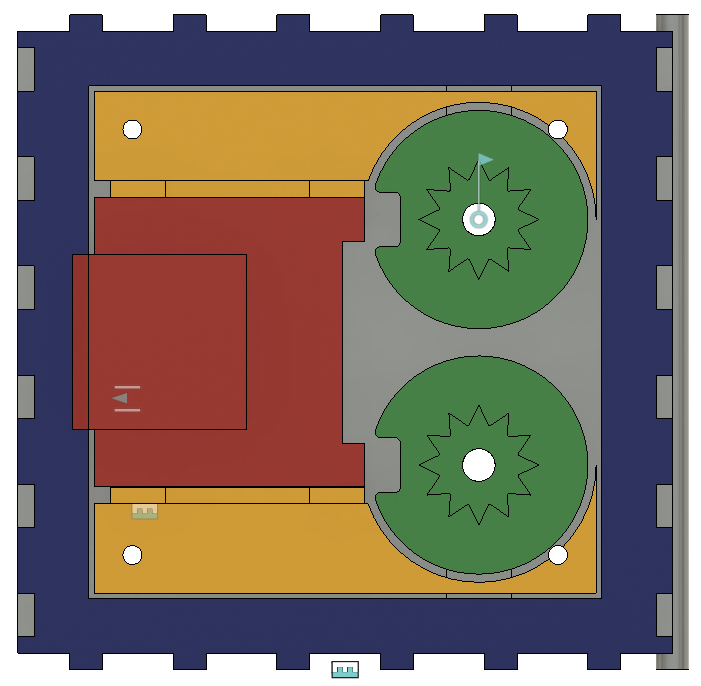
\includegraphics[width=260pt]{kapitoly/obrazky/M1/mechanizmus.png}
    \caption{Zelená barva značí kódovací kola, červená západku, modrá pevnou část trezoru a žluté díly tvoří distanci \centering}
    \label{fig:M1-mechanizmus}
\end{figure}
\newpage